\chapter{Demos clásicas}

\section{Fuego}

\subsection{Investigación inicial}

Una demo que simule un efecto de fuego se podría considerar algo así como el "hola mundo" de la demoscene. Es un ejercicio sencillo con un resultado final bastante espectacular.\\

Tras una búsqueda de información inicial, pude encontrar también dos sitios diferentes en los que se explicaba cómo crear un efecto de fuego.\\ 

En el canal de YouTube de Creature Mann\footnote{\url{https://www.youtube.com/user/kjlg74/featured}} se explica la base teórica para crear un efecto de fuego sencillo\footnote{\url{https://www.youtube.com/watch?v=_SzpMBOp1mE}}. A este vídeo le siguen un par de vídeos de este mismo creador\footnote{\url{https://www.youtube.com/watch?v=iezD8B1ym3w}}\footnote{\url{https://www.youtube.com/watch?v=206TEPBOnLc}} en los que itera sobre el efecto anteriormente creado, añadiendo complejidad (como la posibilidad de controlar la dirección del fuego o trazar un camino que se prende fuego). Por desgracia, los enlaces provistos al código que estos vídeos muestran están caídos, por lo que el código no es accesible. No obstante, la parte argumentablemente más importante, la explicación teórica del efecto, se hace en el primer vídeo.\\

Otra página que ofrece una descripción muy buena del efecto es Lode's Computer Graphics Tutorial\footnote{\url{https://lodev.org/cgtutor/fire.html}}. Esta página sí que aporta código, aunque decidí ignorar la implementación (para evitar que condicionara mi propio desarrollo) y centrarme únicamente en la explicación teórica que se ofrecía, muy similar a la del vídeo anterior aunque más técnica.\\

\subsection{Planteamiento formal}

El fuego es un efecto muy sencillo tanto a nivel teórico como de implementación. Consiste en la convolución de una matriz como la de la figura [\ref{fig:firematrix}] a lo largo de una matriz que tan sólo contiene valores en su fila inferior. Al aplicar esta operación de abajo a arriba, se obtiene un conjunto de valores [\ref{fig:fire_whitegrid}] que al ser asociados a un set concreto de colores [\ref{fig:fire_colouredgrid}], dan una sensación similar al fuego.\\

\begin{figure}
	\begin{equation}
		\begin{bmatrix}
			0 & 0 & 0 \\
			0 & 0 & 0 \\
			\frac{1}{3} & \frac{1}{3} & \frac{1}{3}
		\end{bmatrix}
	\end{equation}
	\caption{Matriz de convolución para generar efecto de fuego}
	\label{fig:firematrix}
\end{figure}

Otra forma de entender esta operación es la siguiente: el valor de cada píxel se deduce de la media del valor de los tres píxeles adyacentes por debajo de él. Para que este efecto se produzca de forma efectiva, la fila inferior de píxeles se suele rellenar con valores aleatorios. De esta forma, la tendencia natural de este modelo es la de disiparse.\\

El único caso en el que no se produciría disipación sería en el que todos los valores de la fila inferior se inicializaran al máximo (en cuyo caso todos los píxeles acabarían con el mismo valor). Para cualquier otra situación, se produce una atenuación progresiva de los valores. 

\begin{figure}[h]
	\centering
	\begin{subfigure}[b]{0.45\textwidth}
		\centering
		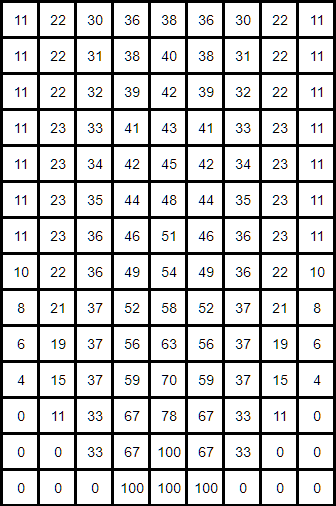
\includegraphics[width=5.09cm]{archivos/fire_whitegrid}
		\caption{Valores resultantes tras convolucionar iterativamente la matriz [\ref{fig:firematrix}] por una matriz de ceros, con valores solo en la fila inferior}
		\label{fig:fire_whitegrid}
	\end{subfigure}
	\begin{subfigure}[b]{0.45\textwidth}
		\centering
		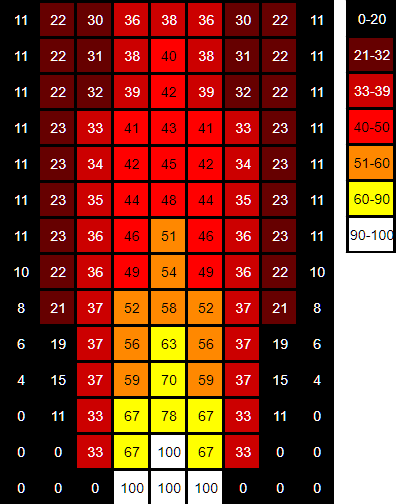
\includegraphics[width=6cm]{archivos/fire_colouredgrid}
		\caption{Efecto resultante de asociar determinados rangos de valores a un set de colores preestablecido}
		\label{fig:fire_colouredgrid}
	\end{subfigure}
\end{figure}

\subsection{Implementación}

Dado el comportamiento descrito, será necesario realizar los siguientes pasos:
\begin{itemize}
	\item Implementar una forma de realizar degradados (o mapas de color)
	\item Reservar e inicializar una matriz a cero, con valores aleatorios en su fila inferior
	\item Implementar el comportamiento de convolución de la matriz [\ref{fig:firematrix}]
\end{itemize}

Para poder crear degradados, se crea la función \emph{GenerateGradient} que dado un conjunto de \emph{ColourStamp} y un tamaño, interpola los valores de colores pasados para generar un degradado continuo en \emph{colourMap}.\\

\begin{lstlisting}[style=C-color, caption={Método para crear gradientes de color},label=cod:generateGradient]
static void GenerateGradient(std::vector<ColourStamp> colours, Pixel* colourMap, int colourMapSize);
\end{lstlisting}

\emph{ColourStamp} (marca de color) es una estructura formada por dos variables: un color y un número decimal (que puede oscilar entre 0 y 1). Este número señala la posición de este color en el gradiente o mapa de color, siendo 0 el inicio y 1 el final. 

\begin{figure}[h]
	\centering
	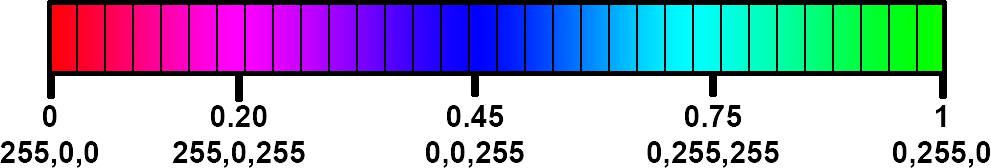
\includegraphics[width=12cm]{archivos/colourGradient}
	\caption{Degradado en 32 celdas dadas 5 marcas de color}
	\label{fig:colourGradient}
\end{figure}

De este modo, si llamamos a la función \emph{GenerateGradient} con los valores para las marcas de color representados en la figura [\ref{fig:colourGradient}] y pasamos un \emph{array} con capacidad para 32 valores, este método producirá un set de colores similar al ilustrado. Esto se hace mediante una interpolación lineal entre los valores que se pasan, creando un degradado de forma progresiva.\\

Una vez tenemos implementado este método, ya podemos crear un degradado de colores de forma sencilla y cómoda, automatizando el proceso de crear un mapa de color para el fuego.\\

Para nuestra implementación, en lugar de asignar a un rango de valores un color específico, asignaremos un color por valor entero. Esto permitirá un resultado más realista, al disponer de una mayor cantidad de colores. Cada celda de nuestra matriz de valores estará formada por un byte. Esto implica que cada celda podrá tener 256 valores distintos, y que por tanto necesitaremos generar un degradado que nos devuelva 256 colores.\\

Creamos un mapa de valores de un byte de tamaño, lo inicializamos a 0 e inicializamos aleatoriamente algunas de las celdas de la fila inferior a su valor máximo (255).\\

\begin{lstlisting}[style=C-color, caption={Creación e incialización del mapa de valores},label=cod:screenMapping,escapechar=|]
screenMapping = new unsigned char[width * height];

for (int i = width * (height - 1), n = width * height; i < n; i++)
{
    if (Fast::Rand() % 10 == 0)|\label{line:fastRand}|
    {
        screenMapping[i] = 255;
    }
}
\end{lstlisting}

Como podemos ver en la línea [\ref{line:fastRand}], hacemos uso de una función propia para la generación de números aleatorios. Esta función está basada en el algoritmo \emph{Xorshift}\footnote{\url{https://en.wikipedia.org/wiki/Xorshift}} de George Marsaglia. La apromaximación usada está basada en una respuesta de \emph{StackOverflow}\footnote{\url{https://stackoverflow.com/questions/1640258/need-a-fast-random-generator-for-c}}.\\

La decisión de usar nuestro propio generador de números aleatorios se debe a que el usualmente provisto por la STL \footnote{\url{https://en.wikipedia.org/wiki/Standard_Template_Library}} es innecesariamente lento y complejo para nuestras necesidades. Para nuestro caso, no necesitamos un algoritmo que pase todos los tests de aleatoriedad\footnote{\url{https://es.wikipedia.org/wiki/Pruebas_de_aleatoriedad}}, con tal de que sea suficientemente "aleatorio al ojo" y sea rápido, nos basta.\\

Una vez hecho esto, tan sólo queda implementar el algoritmo principal, que cree el efecto de fuego sobre el mapa de valores previamente creado, de acorde a la operación descrita en la figura [\ref{fig:firematrix}] y asocie dichos valores con un color generado por la función \emph{GenerateGradient} [\ref{cod:generateGradient}].\\

\begin{lstlisting}[style=C-color, caption={Creación e incialización del mapa de valores},label=cod:simpleFire,escapechar=|]
for (int i = width * (height - 1); i >= 0; i--)
{
    int lowerCell = width + i;|\label{line:simpleFire1}|
    int newCellValue = screenMapping[i] = (screenMapping[lowerCell + 1] + screenMapping[lowerCell] + screenMapping[lowerCell - 1]) / 3.0;|\label{line:simpleFire2}|
    pixels[i] = colourMap[newCellValue];|\label{line:simpleFire3}|
}
\end{lstlisting}

En el código [\ref{cod:simpleFire}] podemos  ver el algoritmo de generación de fuego en su forma más simple. Recorremos la pantalla de abajo a arriba y operamos por cada píxel. En la línea [\ref{line:simpleFire1}] obtenemos, para una posición dada en el mapa de valores, la posición del valor inmediatamente por debajo del mismo. Una vez obtenida esta posición, operamos haciendo la media usando su valor y los adyacentes. Guardamos el resultado como nuevo valor y usamos a la vez este nuevo valor para asociar un nuevo color al píxel en pantalla (línea [\ref{line:simpleFire3}]). Los valores más altos (255) representan tonos blancos y/o amarillentos, mientras que los valores intermedios representarán valores rojizos y los valores más bajos tendrán asociados colores más oscuros.\\

El resultado de aplicar este algoritmo resulta en una imagen estática y de aspecto poco realista [\ref{fig:simpleFire}], pero que ya se empieza a parecer al efecto que buscamos.\\

\begin{figure}[h]
	\centering
	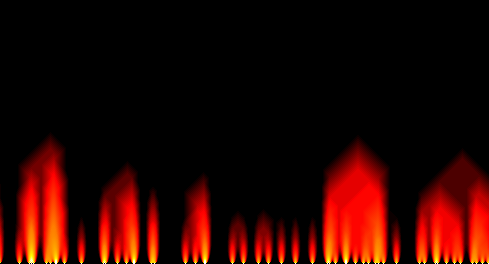
\includegraphics[width=8cm]{archivos/simpleFire}
	\caption{Fuego estático, usando el algoritmo en [\ref{cod:simpleFire}]}
	\label{fig:simpleFire}
\end{figure}

\subsection{Refinamiento}

rgerg
sgsdgsfdh

sg

drga

rg

ergregearg

rgerg

\subsection{Resultado}

rgerg
sgsdgsfdh

sg

drga

rg

ergregearg

rgerg

\section{Geometría}


\subsection{Investigación inicial}

rgerg
sgsdgsfdh

sg

drga

rg

ergregearg

rgerg

\subsection{Planteamiento formal}

rgerg
sgsdgsfdh

sg

drga

rg

ergregearg

rgerg

\subsection{Implementación}

rgerg
sgsdgsfdh

sg

drga

rg

ergregearg

rgerg

\subsection{Refinamiento}

rgerg
sgsdgsfdh

sg

drga

rg

ergregearg

rgerg

\subsection{Resultado}

rgerg
sgsdgsfdh

sg

drga

rg

ergregearg

rgerg


\section{Planos infinitos}

\subsection{Investigación inicial}

rgerg
sgsdgsfdh

sg

drga

rg

ergregearg

rgerg

\subsection{Planteamiento formal}

rgerg
sgsdgsfdh

sg

drga

rg

ergregearg

rgerg

\subsection{Implementación}

rgerg
sgsdgsfdh

sg

drga

rg

ergregearg

rgerg

\subsection{Refinamiento}

rgerg
sgsdgsfdh

sg

drga

rg

ergregearg

rgerg

\subsection{Resultado}

rgerg
sgsdgsfdh

sg

drga

rg

ergregearg

rgerg


\section{Plasma}

\subsection{Investigación inicial}

rgerg
sgsdgsfdh

sg

drga

rg

ergregearg

rgerg

\subsection{Planteamiento formal}

rgerg
sgsdgsfdh

sg

drga

rg

ergregearg

rgerg

\subsection{Implementación}

rgerg
sgsdgsfdh

sg

drga

rg

ergregearg

rgerg

\subsection{Refinamiento}

rgerg
sgsdgsfdh

sg

drga

rg

ergregearg

rgerg

\subsection{Resultado}

rgerg
sgsdgsfdh

sg

drga

rg

ergregearg

rgerg


\section{RotoZoom}

\subsection{Investigación inicial}

rgerg
sgsdgsfdh

sg

drga

rg

ergregearg

rgerg

\subsection{Planteamiento formal}

rgerg
sgsdgsfdh

sg

drga

rg

ergregearg

rgerg

\subsection{Implementación}

rgerg
sgsdgsfdh

sg

drga

rg

ergregearg

rgerg

\subsection{Refinamiento}

rgerg
sgsdgsfdh

sg

drga

rg

ergregearg

rgerg

\subsection{Resultado}

rgerg
sgsdgsfdh

sg

drga

rg

ergregearg

rgerg


\section{Deformaciones de imagen}

\subsection{Investigación inicial}

rgerg
sgsdgsfdh

sg

drga

rg

ergregearg

rgerg

\subsection{Planteamiento formal}

rgerg
sgsdgsfdh

sg

drga

rg

ergregearg

rgerg

\subsection{Implementación}

rgerg
sgsdgsfdh

sg

drga

rg

ergregearg

rgerg

\subsection{Refinamiento}

rgerg
sgsdgsfdh

sg

drga

rg

ergregearg

rgerg

\subsection{Resultado}

rgerg
sgsdgsfdh

sg

drga

rg

ergregearg

rgerg


\section{Túnel de puntos}

\subsection{Investigación inicial}

rgerg
sgsdgsfdh

sg

drga

rg

ergregearg

rgerg

\subsection{Planteamiento formal}

rgerg
sgsdgsfdh

sg

drga

rg

ergregearg

rgerg

\subsection{Implementación}

rgerg
sgsdgsfdh

sg

drga

rg

ergregearg

rgerg

\subsection{Refinamiento}

rgerg
sgsdgsfdh

sg

drga

rg

ergregearg

rgerg

\subsection{Resultado}

rgerg
sgsdgsfdh

sg

drga

rg

ergregearg

rgerg
